\chapter{PATHSAMPLE}
\renewcommand{\pname}{PATHSAMPLE}

\section{Introduction}
\label{sec:intro}

{\tt PATHSAMPLE.2.1} is the current version of the {\tt OPTIM} driver program to implement a
discrete path sampling (DPS) construction of stationary point 
databases and perform kinetic analysis.\cite{Wales02}\cite{Wales03,Wales04,TrygubenkoW06,Wales06}
This implementation provides a number of different methods for growing stationary 
point databases in order to produce samples that are kinetically relevant.
The main difference from {\tt PATHSAMPLE.2.0} is that the geometrical test for
distinguishing stationary points has been changed to use the minimum distance.
This usage is consistent with {\tt OPTIM} and the tolerance is set using the
keyword {\keyw{GEOMDIFFTOL}}. Subsequent enhancements of the code are not implemented
in {\tt PATHSAMPLE.2.0}.

{\tt PATHSAMPLE} relies upon {\tt OPTIM} \cite{optim} to perform geometry optimisation, 
especially double-ended searches for pathways between specified minima. 
In the simplest case, all the {\tt OPTIM} calls will be Dijkstra connect runs
\cite{CarrTW05} (this is the case if the \keyw{CONNECTIONS} parameter is less than or equal to one,
see \S \ref{sec:keywords}).
Please refer to the {\tt OPTIM} documentation for full details of this program \cite{optim}.

The DPS technique is designed to calculate rate constants
between two different regions (A and B) on the potential energy surface, 
where a region is defined by a set of local minima.\cite{Wales02,Wales03,Wales04,TrygubenkoW06,Wales06,
EvansW03b,EvansW04,CarrW05}
In {\tt PATHSAMPLE.2.0} and above, this objective is achieved by building up
a stationary point database using successive double-ended connection runs between
local minima, where connections are chosen according to the minimum distance 
between the minima and their predicted committor probabilities.
Note that that this approach is different from the original philosophy,
which focused upon the rates associated with individual discrete paths and created 
new paths by perturbing old ones.

% <changes>
\section{Recent Changes}
\label{sec:latest}

The {\keyw{NGT}} keyword has been added for a new graph transformation procedure. 
This routine can calculate $k^{\rm SS}$, $k^{\rm NSS}$ and $k^{\rm KMC}$ for both
$A\leftarrow B$ and $B\leftarrow A$, as well as committor probabilities, in one call.
This is now the recommended way to calculate rate constants.

The {\it DIJINIT\/} keyword has been replaced by two separate keywords,
namely {\keyw{DIJINITSTART}\/} and {\keyw{DIJINITCONT}\/}, to simplify the generation of
initial paths. 

{\keyw{DIJINITSTART}\/} is intended for automatic setup of the {\tt min.A}, {\tt min.B},
{\tt min.data}, {\tt ts.data}, {\tt points.ts} and {\tt points.min} files from initial
{\tt odata.start} and {\tt odata.finish} files. In contrast to the previous 
philosophy, {\keyw{DIJINITSTART}\/} will {\bf overwrite database files if they already exist}.
Hence it is possible to wipe an existing database with this keyword.

{\keyw{DIJINITCONT}\/} is intended for continuation of initial path searches that have not yet 
completed. It can also be used to start a run if the required database entries for two
end points have been created by hand. {\keyw{DIJINITCONT}\/} will check that the required
files are present in the current working directory, and stop if they are not.

The MFPT calculation for the fastest steady-state path (ignoring recrossings)
in a {\keyw{DIJKSTRA}} calculation
has been changed to the graph transformation approach.\cite{TrygubenkoW06}

The printing of rate constants at the end of a {\keyw{GT}\/} calculation has been changed
to make it clear which values are calculated assuming that detailed balance holds.
An extra summary line with the non-detailed balance rate constants is printed at the end.

After each cycle over the available CPU's {\tt PATHSAMPLE} will now check to see if the
file {\tt pathdata.change} exists in the current working directory. 
If it does, then {\tt pathdata.change} is copied to {\tt pathdata}
and all parameters are reread using {\bf keyword}.
This feature is designed to allow for change of parameters during a run without
the need to kill and requeue a job. 
Attempts to change variables that affect declarations of array bounds will 
cause the program to crash.

%</changes>
\section{Input files}
\label{sec:input}
The following files are required in the directory where {\tt PATHSAMPLE} is executed.
\smallskip
\begin{itemize}
\item {\tt pathdata}: contains parameters to control the stationary point
sampling and/or the kinetic analysis. See \S\ref{sec:keywords}.
\item {\tt odata.*} files: the {\tt odata} file is the control file for {\tt OPTIM}. 
One {\tt odata} file is
needed for each type of {\tt OPTIM} job performed by {\tt PATHSAMPLE}. See \S\ref{sec:odatafiles}.

\item {\tt commit.data}. This file is updated every time a committor probability 
calculation is performed. Initial committor probabilities are read from it if the
file is detected. Otherwise, the initial values are 
set to zero and one as appropriate.
If a {\tt PATHSAMPLE} run ends abnormally it is possible for the number of entries
in {\tt commit.data} to be less than the number of local minima in {\tt min.data}.
In this case the missing values are automatically
set to zero. This procedure does not work with some compilers
if they behave incorrectly on reaching the end of file.
In this case the missing zeros can simply be added using a text editor.

\end{itemize}

The following files may be required, depending upon the keywords set in {\tt pathdata}:
\smallskip
\begin{itemize}
\item {\tt min.A}, {\tt min.B} and {\tt min.data}: lists of A, B and intermediate minima, respectively. 
The first line of {\tt min.A} is the number of A minima (free format), $N_{\rm A}$; on the following lines
there must be $N_{\rm A}$ integers (free format), which specify all the local minima 
belonging to the A set. Hence, the A region can be changed simply by editing this file.
{\tt min.B} has the same format for the B minima.
The numbering of the local minima must be consistent with the order of their
coordinates in {\tt points.min} (see below).
However, unlike older versions of {\tt PATHSAMPLE}, the A and B minima can appear 
in any order, facilitating regrouping schemes.
The file {\tt min.data} has the format:

{\it energy\quad frequency\quad pgorder\quad itx\quad ity\quad itz}

for each minimum, where $energy$ is the potential energy (as calculated by {\tt OPTIM}), 
$frequency$ is the natural log of the
product of positive eigenvalues from the mass-weighted Hessian
(used to evaluate partition functions and rates constants), $pgorder$ is the order of the point group,
and $itx, ity, itz$ are the (sorted) eigenvalues of the inertia tensor.
The order of entries in {\tt min.data} must agree with the {\tt min.A},
{\tt min.B} and {\tt points.min} files.

\item The file {\tt ts.data} is analogous to the {\tt min.data} file, 
but contains data for the transition states. The format is: 

{\it energy\quad frequency\quad pgorder\quad min1\quad min2\quad itx\quad ity\quad itz} 

where the entries are the same as for the minima, with the addition of {\it min1} and
{\it min2}, which identify the minima that the transition state connects. 
This file must be consistent with {\tt points.ts} (see below).

\item {\tt points.min}: contains the Cartesian coordinates of all the minima that are specified in 
{\tt min.data} in the same order. It is 
an unformatted direct access file, written with the Fortran specifier 
{\tt RECL=8*3*NATOMS}. 

\item {\tt points.ts}: as for {\tt points.min}, but contains the transition state 
coordinates.

\item {\tt nodes.info}: must be present for runs on a distributed memory machine.
The first line must contain an integer equal to the number of nodes available,
and the names of these nodes must follow below. 
On the final line the userid must be provided.
An example script for the qsub command could look like:
\begin{table}[H]
\begin{center}
\begin{tabular}{l}
\#!/bin/csh \\
\#PBS -q h4 \\
cd \$PBS\_O\_WORKDIR \\
cat \$PBS\_NODEFILE $>$\& output \\
wc output $>$ nodes.info \\
cat \$PBS\_NODEFILE $>>$ nodes.info \\
echo \$USER $>>$ nodes.info \\
/home/bin/pathsample $>>$\& output \\
\end{tabular}
\end{center}
\end{table}

\item {\tt path.info.startup}: an {\tt OPTIM} {\tt path.info}
file from a connect run that connects an A minimum to a B minimum.
Note that an output file is not required, unlike older versions of {\tt PATHSAMPLE}.
This file is needed to
provide an initial path, and the file name startup is specified in the {\tt pathdata} file
by the {\keyw{STAR}TFROMPATH} keyword.
If the files {\tt min.A} and {\tt min.B} are absent, then {\keyw{STAR}TFROMPATH}
will create them, with a single minimum specified in each region, corresponding
to the entries specified on the {\keyw{STAR}TFROMPATH} line after the file extension
startup.
The rest of the minima read from the
{\tt path.info.startup} file will be placed in the intervening set.
Note that for {\tt path.info} files in the new {\tt OPTIM}
{\keyw{DUMP}ALLPATHS} format, the two end point minima will generally not
be the first and last entries.
Since {\tt min.data} contains only unique minima, whereas the {\tt path.info} file may have
duplicates, the positions of the starting and finishing minimum may not be obvious.
A quick way to check these values is to run {\tt PATHSAMPLE} first with {\keyw{CYCLES} 0},
find the positions of the two minima in {\tt min.data} and correct
the values in {\tt pathdata}, remove {\tt min.*}, {\tt points.*}
and {\tt *.data}, and start the real {\tt PATHSAMPLE} run.
If the {\tt path.info.startup} file is in the new {\keyw{DUMP}ALLPATHS} format
then {\tt pathdata} must contain the keyword {\keyw{STAR}TTRIPLES}.
For a setup where the A and B sets are predefined in {\tt min.A} and {\tt min.B}
a connecting pathway can be read using the keyword {\keyw{ADDPATH} add} in {\tt pathdata}.
A path will then be read from file {\tt add}; if this path is
in the new {\keyw{DUMP}ALLPATHS} format then the keyword {\keyw{ADDTRIPLES}} must
be present in {\tt pathdata}.
\end{itemize}

The {\tt min.data}, {\tt ts.data}, {\tt points.min} and {\tt points.ts} files are 
updated by {\tt PATHSAMPLE} as new minima and transition states are found. 

\section{Keywords: the {\tt pathdata} file}
\label{sec:keywords}
Input is keyword driven with sensible defaults in most cases. See the source {\bf keyword.f} if in doubt.
The following keywords are recognised, where {\it n\/}, {\it x\/} and {\it a\/} are integer,
real and character data, respectively. A line beginning with {\it COMMENT} is ignored.
\smallskip

\subsection{A}

\ksec{ADDPATH}{ afile \/}: reads pathway data from file {\tt afile}. If this 
file is in {\keyw{DUMP}ALLPATHS} format then the keyword {\keyw{ADDTRIPLES}} is also needed.


\ksec{ADDPERM}{\/}: adds permutational isomers of every 
stationary point to the databases. Not recommended except for small systems
where you are using a tagged atom to study an isomerisation (e.g. 2D LJ7).

\ksec{ADDTRIPLES}{ \/}: specifies that the {\tt afile} file to be read
according to the {\keyw{ADDPATH} afile} keyword is in 
{\keyw{DUMP}ALLPATHS} format.

\ksec{ANGLEAXIS}{ \/}: specifies angle-axis coordinates for rigid bodies.

\ksec{AMH}{ \/}: specifies an AMH potential.

\ksec{AMHQ}{ whichmin \/}: Calculates Wolynes Q score based on the native state structure.

\ksec{AMHRMSD}{ whichmin \/}: Calculates RMSD based on the native state structure.

\ksec{AMHQCONT}{ whichmin rcut \/}: Calculates Q-cutoff score based on a native distance. 

\ksec{AMHRELQ}{ whichmin1 whichmin2 \/}: Calculates Wolynes Q score between two minima. 

\ksec{AMHALLATOM}{ \/}: Adds sidechains and completes backbone for AMH structures with SCWRL. 
Input structure is amhmin.pdb. Output structure is amhmin.pdb.scwrl. Scwrl output logs scwrl\_out.

\ksec{AMH\_RELCO}{whichmin rcut \/}: Calculates relative contact order for AMH structures.

% \ksec{BREADTH}{\/}: breadth-first analysis to find the shortest A$\leftrightarrow$B paths.
% {\bf Not implemented yet}.

\subsection{B-C}
\ksec{BHINTERP}{ dthresh maxe bhsteps conv T stepsize accrat K sfrac ICINTERP\/}: specifies that
{\tt OPTIM} jobs should be run using only the {\keyw{BHINTERP}} interpolation option,
where no transition state searches are run. Requires the auxiliary file {\tt odata.bhinterp}.
This option is intended for use with {\keyw{DIJINITSTART}} and {\keyw{DIJINITCONT}}.
The various arguments are used to add a {\keyw{BHINTERP}} line to the {\tt OPTIM} {\tt odata} file.
The distance threshold parameter specifies that interpolation between consecutive minima
in the Dijkstra list should occur if their minimum distance is greater than {\it dthresh}. 
The threshold actually used in the corresponding {\tt odata} file is either the minimum distance
divided by two or {\it dthresh}, whichever is greater. This arrangement enables 
parallel {\tt OPTIM} jobs to be run for different pairs of minima.
Intermediate minima are only accepted if their energy is below {\it maxe}.
A basin-hopping global optimisation run of {\it bhsteps} is run for each pair of
end point minima within {\it dthresh\/} using an RMS gradient convergence criterion
of {\it conv\/}, a temperature parameter of {\it T\/}, and a maximum step size for
perturbations of {\it stepsize\/}. The step size is adjusted dynamically towards an
acceptance ratio target of {\it accrat\/}.  
The objective function consists of the energy of the minimum on the potential energy surface
plus the energy corresponding to harmonic springs of force constant {\it K\/} 
stretched to displacements corresponding to the minimum distance between the new minimum
and the end points.
{\it sfrac\/} is used in the initial interpolation: a value of 0.5 will put the initial
guess half-way between the end points, and in general the geometry will be {\it sfrac\/} times one
end point plus $(1-${\it sfrac\/}$)$ times the other.
For large distances, using a value other than a half may be helpful.
If {\it ICINTERP\/} is present then amino acid side chains are interpolated using
internal coordinates for CHARMM runs.
The step size is interpreted in degrees for CHARMM, where the perturbations used
to step between minima are performed using dihedral angle twists.
The algorithm is applied recursively between minima as new minima are found.
A new minimum will not be accepted if both distances to the minima we are
currently trying to interpolate between are greater than the minimum distance
between these minima.

\ksec{BISECT}{ dthresh maxe bisectsteps attempts ICINTERP\/}: specifies that
{\tt OPTIM} jobs should be run using only the {\keyw{BISECT}} interpolation option,
where no transition state searches are run. Requires the auxiliary file {\tt odata.bisect}.
This option is intended for use with {\keyw{DUMMYTS}}.
The various arguments are used to add a {\keyw{BISECT}} line to the {\tt OPTIM} {\tt odata} file.
The distance threshold parameter specifies that bisection between consecutive minima
is attempted if their minimum distance is greater than {\it dthresh}. 
The interpolated geometry is minimised and compared with the starting structures.
New minima are only accepted if their energy is below {\it maxe}; they are added to the
current list of known minima in the {\tt OPTIM} job between the two starting structures.
The estimated energy of any dummy transition states between the two starting structures
is raised if the sum of distances between the new minimum and the two structures is
greater than the original minimised distance.
{\it bisectsteps\/} is the maximum number of bisection steps, and
{\it attempts} is the number of attempts per step for a given pair.
If minimisation leads to one of the end points the interpolation is changed to use 
fractions of the two structures that become increasingly skewed, as for
the adjustment of {\it sfrac\/} with {\keyw{BHINTERP}\/}, above.
The {\tt ts.data} file is rewritten if the any dummy transition state energies are revised.
If {\it ICINTERP\/} is present then amino acid side chains are interpolated using
internal coordinates for CHARMM runs.

\ksec{BULK}{ x1 x2 x3\/}: a bulk system in a periodic box of lengths {\it x1, x2, x3\/}.

\ksec{CALCORDER}{\/}: the program will call subroutine {\bf calcorder.f90} and calculate
order parameters, before exiting. Since the order parameters will be system dependent 
users must compile in an appropriate {\bf calcorder.f90} themselves.

\ksec{CAPSID}{ rho eps rad h\/}: parameters for a rigid pentagonal pyramid. If $h$ is omitted
it is set to half $rad$ by default.

\ksec{CHARMM}{ n\/}: specifies that the CHARMM potential is used in the {\tt OPTIM} runs.
{\it n} is an integer used in {\bf perturb.f} and {\bf tssearch.f} to perturb dihedral angles
if additional single-ended transition state searches are needed.

\ksec{CHECKCONECTIONS}{\/}: instruction to check that each minimum has at least the number
of connections specified by the {\keyw{CONNECT}IONS\/} keyword at the start of every run,
before anything else is done. See {\keyw{CONNECT}IONS\/} below.

\ksec{CLOSEFILES}{\/}: open and close the {\tt min.data} and {\tt ts.data} files as needed.
By default these files stay open all the time. For small systems this inevitably seems to cause
file corruption on nfs mounted file systems, which is apparently due to bugs in the interaction
of nfs with the Linux kernel. The symptom is that strings of control characters appear randomly in
{\tt min.data} and/or {\tt ts.data}, which means that the run cannot continue without
manually fixing the file in question.
The {\tt CLOSEFILES} keyword has provided a successful workaround for this problem.

\ksec{CONNECTIONS}{ n maxattempts\/}: minimum number of connections for each minimum. 
For each new minimum found {\tt PATHSAMPLE} will attempt to find {\it n\/} connected minima.
If {\it n} is one or fewer then no additional single-ended transition state searches are
needed, and the more efficient {\bf cycle2.f90} subroutine is used. In this case, {\tt OPTIM}
jobs do not have to be processed in batches; instead, a new {\tt OPTIM} job is submitted
as soon as one finishes. The default for {\it n} is now 0.
The maximum number of transition state searches from each new minimum is {\it maxattempts}, 
for which the default is 10.
Note that you will need files {\tt odata.tssearch} and {\tt odata.path} in the current
working directory if {\it n} is greater than one.

\ksec{CONNECTREGION}{ min1 min2 dist\/}: grows the stationary point database by running
double-ended transition state searches between minima whose minimum separation is less then
{\it dist}. {\it min1} and {\it min2} specify the starting minima in the double loop over
pairs, so that restarted runs need not consider pairs that have previously been searched.
Minima that already have a direct connection are ignored.
The maximum number of candidate pairs calculated per call to {\bf connectd.f90} is 10000.
This parameter may be useful for exhaustive searches for small systems.

\ksec{COPYFILES}{ a1 a2 a3 $\ldots$\/}: specify additional files that need to be
copied to distributed nodes. Only files {\tt odata.<pid>} and {\tt finish.<pid>} are
copied by default. For example, the BLN potential requires file {\tt BLN sequence}, while
CHARMM runs may need one or more {\tt crd} files. Each string must be less than or equal to
twenty characters in length, and the total, including separating blanks, must not exceed
80 characters. If the {\keyw{CHARMM}\/} keyword is set and the {\keyw{COPYFILES}\/} 
arguments do not include {\tt input.crd} then the program will stop.

\ksec{COPYOPTIM}{\/}: if present, some of the {\tt OPTIM} output files will be copied to
the mother superior node and not deleted. This behaviour also occurs if the {\keyw{DEBUG}\/}
keyword is present. The copied files, in addition to {\tt path.info} ({\tt min.data.info} 
for a {\keyw{BHINTERP}\/} run), are the {\tt OPTIM} output file, the {\tt odata} file
and the {\tt finish} file.

\ksec{CPUS}{ ncpu}: specifies the number of cpu's available on an SMP machine. If used on
a distributed memory cluster then {\it n} {\tt OPTIM} jobs will be submitted on one node.
Can be used to run multiple jobs on an interactive testing node of a distributed memory
machine.

\ksec{CYCLES}{ n}: the number of cycles of {\it ncpu} or
{\it jpn}$\times$nodes {\tt OPTIM} jobs to run in sampling the stationary point
database.

\subsection{D-E}
\ksec{DEBUG}{\/}: turn on debug printing.

\ksec{DGT}{ DisconnectSources AltPbb Rescale Normalise\/}: 
dense optimised graph transformation rate calculation \cite{TrygubenkoW06}.
The four arguments are all logicals, so an example input line might look
\vbox{DGT T T F F}. If true (the default) {\it DisconnectSources} specifies that
a full transformation should be performed for each source, disconnecting the 
other sources. The resulting rate constants correspond to the KMC result and
$k^{\rm KMC}$ \cite{Wales06}.
If {\it AltPbb\/} is true (default is false) then additional work is done to
maintain precision, which roughly doubles the execution time, but may be needed at low
temperature.
If {\it Rescale} is true (default false) an alternative strategy is used 
to try and prevent error propagation.
Setting {\it Normalise} true (default false) instructs {\tt GT2input.f90} to check the normalisation
of branch probabilities. This should not be necessary.

\ksec{DIJINITCONT}{ exp or n\/}: continue an initial Dijkstra connection 
from information in the existing {\tt min.A}, {\tt min.B}, {\tt min.data},
{\tt ts.data}, {\tt points.ts} and {\tt points.min} files.
The minimum information required consists of database entries 
for the two endpoint minima.
The algorithm used is similar to {\tt OPTIM}, except that the missing connections can
be sought in parallel {\tt OPTIM} runs, each of which is itself a separate
Dijkstra connect calculation.
If {\it exp} appears after {\it DIJINIT\/} then the edge weights are based on the
exponential distance; otherwise the distance is raised to the power {\it n}, which
defaults to 2.
If the same connection is attempted more than once the same {\tt odata} file
is used, and the previous calculation is simply duplicated.
The number of parallel searches is equal to the number of processors available.
For the first cycle all the searches would be the same, because there must be a single 
gap between the two end minima.
To avoid unnecessary duplication it is best to perform an initial run on
one processor, or a single node, for one cycle (see {\keyw{DIJINITSTART}\/} below). 
Then restart by simply increasing the number of cycles in the {\tt pathdata} file
as well as the number of processors.
In the Dijkstra analysis minima with zero connections are removed. 
This value can be changed using a {\keyw{DIJKSTRA} n} line in {\tt pathdata}.

\ksec{DIJINITCONTFLY}{ exp or n\/}: performs the same function as {\keyw{DIJINITCONT}} but
calculates distances between local minima on the fly. This approach may be necessary 
for initial path runs that produce more that 20,000 minima, where fitting all the 
distances into memory becomes an issue.

\ksec{DIJINITSTART}{ exp or n\/}: perform an initial Dijkstra connection run 
for the two endpoints specified in {\tt odata.start} and {\tt odata.finish}. 
In this case the files {\tt min.A}, {\tt min.B}, {\tt min.data}, {\tt ts.data} (and all
points files) will be created automatically.
{\bf Any existing database information will be overwritten}.
Note that the {\tt odata.start} and {\tt odata.finish} files must contain
the {\tt OPTIM} keyword {\keyw{DUMP}DATA\/} and calculate the normal mode frequencies.
For a CHARMM run the files {\tt start.crd} and {\tt finish.crd} are also needed.
The algorithm used is similar to {\tt OPTIM}, except that the missing connections can
be sought in parallel {\tt OPTIM} runs, each of which is itself a separate
Dijkstra connect calculation.
If {\it exp} appears after {\it DIJINIT\/} then the edge weights are based on the
exponential distance; otherwise the distance is raised to the power {\it n}, which
defaults to 2.
If the same connection is attempted more than once the same {\tt odata} file
is used, and the previous calculation is simply duplicated.
The number of parallel searches is equal to the number of processors available.
For the first cycle all the searches will be the same, because there must be a single 
gap between the two end minima.
To avoid unnecessary duplication it is usual to perform the first cycle of an initial
connection attempt on one processor for one cycle. 
Then restart using {\keyw{DIJINITCONT}\/} 
by simply increasing the number of cycles in the {\tt pathdata} file
as well as the number of processors.
For the first cycle it is also a good idea to use just one double-ended connection
cycle in {\tt odata.connect}, and increase this value on subsequent cycles
when some intervening minima are known. 
Otherwise the first {\tt OPTIM} job may spend a great deal of time performing
connection attempts that could be spread over multiple processors in a
{\tt PATHSAMPLE} {\keyw{DIJINITCONT}\/} job.
In the Dijkstra analysis minima with zero connections are removed. 
This value can be changed using a {\keyw{DIJKSTRA} n} line in {\tt pathdata}.

\ksec{DIJINITSTARTFLY}{ exp or n\/}: performs the same function as {\keyw{DIJINITSTART}} but
calculates distances between local minima on the fly. This approach may be necessary 
for initial path runs that produce more that 20,000 minima, where fitting all the 
distances into memory becomes an issue.

\ksec{DIJKSTRA}{ n\/}: perform a Dijkstra analysis to find the path
with the largest contribution to the `SS' rate constant ignoring recrossings. Minima with
{\it n} connections or fewer are pruned.
If {\keyw{REGROUP}FREE}, {\keyw{REGROUP}RATE}, or {\keyw{REGROUP}PE} is present
in {\tt pathdata} then the stationary points will be regrouped first. In this
case the energies in {\tt Epath} are free energies, and files such as
{\tt redopoints} and {\tt stationary.points} are not produced.
Once a path is found the rate corresponding to that path in isolation,
i.e.~ignoring other connections, is calculated using the graph transformation
method.\cite{TrygubenkoW06}.

\ksec{DIJKSTRAWAIT}{\/}: perform a Dijkstra analysis to find the path
with the lowest sum of waiting times times initial conditional probability.

\ksec{DIJPAIR}{ n1 n2 string\/}: choose pairs of minima for connection attempts based on
the highest barrier on the path that makes the largest contribution
to the `SS' rate constant. The first time a given transition state is the highest,
the connection attempt is between the adjacent minimum.
The next time it is chosen we use the second-nearest neighbours along the path in question.
The parameter {\it n1} determines how many steps away from the transition state we
continue these connection attempts for. The default is {\it n1}=1.
Once {\it n1\/} attempts have been tried for the highest transition state we
move to the second-highest, and so on.
Minima with {\it n2} connections or fewer are iteratively removed before the network
analysis. The default value for {\it n2} is one.
The {\it string\/} argument, which is optional, only has an effect if it is the
word `BARRIER'. In this case the pairs of minima to connect are sorted according to the 
largest barrier 
that separates them. Otherwise they are sorted in order of increasing
energy of the minimum that is separated from the product region.

\ksec{DIRECTION}{ a\/}: the direction (`AB' or `BA') determines the sense in which KMC trajectories
are run for {\keyw{KMC}} and {\keyw{KMC}commit}. It also determines which state is the target
in committor probability calculations. 

\ksec{DSCALE}{ x\/}: specifies how the separation between local minima, {\it d}, is used
to select the pair used in the next attempted connection. If
$\exp(-(d-x)/x) < $ a random number drawn from $[0,1]$ then the distance criterion is accepted.
There is also a criterion for the difference in committor probabilities (see {\keyw{PSCALE}}).
If $d<x$ then the distance criterion is always satisfied; above $x$ the probability
of acceptance decreases exponentially.

\ksec{DUMMYRUN}{\/}: specifies that no {\tt OPTIM} jobs should be submitted; the program just
sleeps instead.

\ksec{DUMMYTS}{\/}: specifies that dummy transition state entries should be created for
selected pairs of minima. The corresponding database of minima and dummy transition states
can be refined using any of the usual schemes, e.g.~{\keyw{SHORTCUT}\/}, {\keyw{FREEPAIRS}\/}, etc.
Either {\keyw{BHINTERP}\/} or {\keyw{BISECT}\/} needs to be specified in the {\tt pathdata} file,
so that {\tt OPTIM} jobs only locate new local minima and feed them to {\tt PATHSAMPLE}
via {\tt min.data.info} files.
The dummy entries in {\tt ts.data} include connections for all nearest pairs of minima
for {\keyw{BHINTERP}\/}, but only for successive pairs of minima with {\keyw{BISECT}\/}.
The dummy energy and log product of mass-weighted Hessian eigenvalues for each
{\tt ts.data} entry are chosen according to properties of the two minima.
The current energy estimate is the energy of the higher minimum plus the minimum distance
between the two minima.
The estimate for the log product of eigenvalues simply rescales the value for the higher minimum,
effectively removing one degree of freedom.
At some point a decision must be made to start linking the minima via genuine transition
states. To do this we use {\keyw{USEPAIRS}}, which reads a sequence of stationary points in
the format of the {\tt Epath} file.
The dummy {\tt ts.data} and {\tt pairs.data} files must be renamed or removed.

\ksec{DUMPGROUPS}{\/}: specifies that the groups of potential energy minima and transition
states corresponding to groups of free energy minima and transition states should be dumped
to files {\tt minima\_groups} and {\tt ts\_groups} following regrouping.

\ksec{EDIFFTOL}{ x\/}: two stationary points will only be identified as the
same structure if their energy difference is less than {\it x} and their minimum
distance is less than the threshold specified by {\keyw{GEOMDIFFTOL}\/}.
{\keyw{ETOL}\/} specifies the same parameter and is provided for backward compatibility.

\ksec{ENERGY}{ x\/}: specifies that the microcanonical ensemble at energy {\it x\/} is to be used
to calculate rate constants. Mutually exclusive with {\keyw{TEMPERATURE}\/}.

\ksec{ETOL}{ x\/}: energy difference criterion for distinguishing stationary points. 
Used with {\keyw{ITOL}\/} in {\tt PATHSAMPLE.2.0\/} and {\keyw{GEOMDIFFTOL}\/} in
{\tt PATHSAMPLE.2.1\/}. {\keyw{EDIFF}TOL\/} specifies the same parameter.

\ksec{EVCUT}{ x\/}: tolerance for Hessian eigenvalues or frequencies read from
a {\tt path.info} file by the {\bf getallpaths} subroutine.
If an eigenvalue is detected that should belong to the positive set by lies below
{\it x\/} (default value $2\times10^{-6}$) the min-sad-min triple is skipped.

\ksec{EXEC}{ a\/}: name of the {\tt OPTIM} executable to be called by {\tt PATHSAMPLE}.

\ksec{EXTRACTMIN}{ n\/}: extract the coordinates of minimum {\it n} from
{\tt points.min} and write them to file {\tt extractmin}. If the {\keyw{CHARMM}}
keyword is present then a pdb format {\tt extractedmin.pdb} will also be
produced. If $n\le0$ then all the minima are extracted to {\tt extractmin}.

\ksec{EXTRACTTS}{ n\/}: extract the coordinates of minimum {\it n} from
{\tt points.ts} and write them to file {\tt extractts}.
If the {\keyw{CHARMM}}
keyword is present then a pdb format {\tt extractedts.pdb} will also be
produced. If $n\le0$ then all the transition states are extracted to {\tt extractts}.

\subsection{F-K}
\ksec{FREEPAIRS}{ x1 x2 x3\/}: connection pairs are chosen based upon the same free energy
regrouping scheme as {\keyw{REGROUP}FREE\/}.
{\it x1} corresponds to the free energy barrier height below which free energy
minima are combined.
Free energy minima that lie more than {\it x2} units of energy above the global
free energy minimum group are ignored.
{\it x3} is the energy increment used in the superbasin analysis to estimate 
barriers.
Pairs of potential energy minima are chosen from groups based on the ratio
of free energy barrier height to product divided by free energy difference
from product. Hence we highlight groups that correspond to {\it frustration\/},
with similar energies to the product but high barriers.
Local minima from these free energy groups are then chosen
based upon an additional shortest distance criterion. 
Searches are not repeated for the same potential energy minima.
{\bf NOTE}: for this to work efficiently it is important to have the lowest
minima specified in {\tt min.A} and {\keyw{DIRECTION}\/} set to AB, so that
the A minima are product, and lie at the bottom of the landscape.
See also the {\keyw{PAIRLIST}\/} keyword.

\ksec{FREEZE}{ n1 n1\ldots\/}: specifies that atoms $n1$, $n2\ldots$, should be frozen.
This keyword must come after the {\keyw{NATOMS}\/} keyword.

\ksec{FRICTION}{ $\gamma$\/}: specifies that rate constants should be 
calculated using the multi-dimensional version of Kramer's theory described by
Berezhkovskii, Pollak and Zitserman.\cite{BerezhkovskiiPZ92}
$\gamma$ is a phenomenological `friction' coefficient in frequency units, which
must correspond to the units for the Hessian eigenvalue product in the
{\tt ts.data} file. This formulation requires the imaginary normal mode
frequency for each transition state, and the {\tt ts.data} file must therefore
contain a ninth column corresponding to the unique negative Hessian eigenvalue.
For the {\keyw{CHARMM}\/} and {\keyw{AMBER}\/} force fields this eigenvalue is the
angular frequency squared in SI units, while for all other potentials it will
be in reduced units. Such databases can be extended without using the `friction'
formulation by setting the {\it IMFRQ\/} keyword (or by using $\gamma=0$).

\ksec{GEOMDIFFTOL}{ x\/}: two stationary points will only be identified as the
same structure if their minimum separation is less than {\it x} and their energy
difference is less than the threshold specified by {\keyw{EDIFFTOL}\/}.

\ksec{GT}{ n1 n2\/}: specifies that the graph transformation approach\cite{TrygubenkoW06}
should be used to calculate rate constants. 
Minima with {\it n1} connections or fewer are iteratively removed before the rate
calculation. {\it n2} specifies that the rates should be calculated every {\it n2} cycles
during the refinement of the stationary point database. For large databases making {\it n2} equal to one
could slow the sampling down significantly.
To run a GT calculation without changing the stationary point database set {\keyw{CYCLES} 0}.
See keyword {\keyw{GT2}\/} for a more general implementation of graph transformation.
The rates produced from the {\keyw{GT}} keyword correspond approximately to the
$k^{\rm NSS}$ rate constants \cite{TrygubenkoW06,Wales06}.
Branching probabilities for return to the same initial state are set to zero,
and all the other connections are renormalised accordingly. Hence the final branching
probabilities for a given source include arbitrary revisits to that source before 
a path reaches a different source or a product, so they do not quite correspond to 
committor probabilities. In practice, the resulting rate constants generally seem to
be close to the $k^{\rm NSS}$ values.

\ksec{GT2}{} This keyword has been removed. Please use {\it SGT},
{\it DGT} or {\keyw{SD}GT}.

\ksec{GT}{2RSwitch x \/}: specifies that the generalised graph transformation
routines switch from single to double precision when the density reaches {\it x\/}.
The default value is $x=0.08$.
See keyword {\keyw{SD}GT\/} and subroutine {\bf GT2} for more information. 

\ksec{GT}{2PTOL x\/}: specifies the threshold for deciding that a node is dead
in the generalised graph transformation routines. The default value is $x=0.00001$.

\ksec{IMFRQ}{\/}: specifies that the {\tt ts.data} file should contain a ninth 
column containing the unique negative Hessian eigenvalue. This
is the eigenvalue corresponding to the imaginary normal mode frequency.
See also the {\keyw{FRICTION}\/} keyword, which implies the same format for
{\tt ts.data} and calculates the rate constants using a phenomenological
description of dynamical solvent friction.

\ksec{ITOL}{ x\/}: principal moment of inertia tensor difference criterion for 
distinguishing stationary points. All three values are compared for stationary points
in the initial setup phase. However, unlike {\tt PATHSAMPLE.2.0}, the alternative
criterion specified by {\keyw{GEOMDIFFTOL}\/} is used to distinguish stationary points
in {\tt PATHSAMPLE.2.1}.

\ksec{JOBSPERNODE}{ jpn\/}: specifies the number of jobs to run on each node for a
calculation on a distributed memory machine. The number of nodes and their
identities must be defined in the job submission script in the {\tt nodes.info} file.

\ksec{KMC}{ n1 x n2\/}: perform {\it n1} KMC runs having iteratively removed
minima with {\it n2} connections or fewer.
{\it x} specifies a pair threshold for the product, {\it p}, of forward and backward
branching probabilities between two minima.
If {\it p} is greater than {\it x} then a leapfrog move will be attempted to a
different connected minimum when either of the pair is encountered.
Setting {\it p} to one or more means that leapfrog moves will not be used.
No additional stationary points will be calculated in a {\keyw{KMC}}
run: the {\keyw{CYCLES}} keyword is ignored if it is present in {\tt odata}.
Only one of the {\keyw{GT}}, {\keyw{GT}2}, {\keyw{KMC}} and {\keyw{KMC}commit} keywords should be
present in a given {\tt pathdata} file.

\ksec{KMC}{commit n1 x1 x2 x3 x4 n2}: specifies a rate constant calculation using
committor probabilities and appropriate waiting times. This subroutine can calculate 
both `SS' and `NSS'-type rate constants.\cite{TrygubenkoW06}
{\it n1} is the number of KMC trajectories to run. If {\it n1} is zero then
the waiting time in a given minimum is the the escape time
to its connected neighbours. Combined with the committor probabilities,
these waiting times give `SS' rate constants. If {\it n1} is greater than zero then
the waiting times are calculated for KMC runs that terminate as soon as they reach
a minimum in either the A or the B region. The resulting rate constants
are described as `NSS'.\cite{TrygubenkoW06}
{\it x1} is the maximum number of iterations allowed in the committor probability
calculation; it is a real number because the value required may exceed the size allowed
for an integer.
{\it x2} is a convergence condition for the committor probabilities, and is defined
in terms of the percentage change between iterations.
{\it x3} is the $\omega$ parameter used in the successive overrelaxation calculation
of the committor probabilities. It should be greater than or equal to one, but less than 2.
The default value is one, which results in Gauss-Seidel iterations.
{\it x4} specifies a pair threshold for the product, {\it p}, of forward and backward
branching probabilities between two minima.
If {\it p} is greater than {\it x} then a leapfrog move will be attempted to a
different connected minimum when either of the pair is encountered.
Setting {\it p} to one or more means that leapfrog moves will not be used.
{\it n2} determines the minimum connectivity allowed for local minima to be
admitted into the calculation. The minima are iteratively pruned to remove those
with {\it n2} connections or fewer.
No additional stationary points will be calculated in a {\keyw{KMC}commit}
run: the {\keyw{CYCLES}} keyword is ignored if it is present in {\tt odata}.
Only one of the {\keyw{GT}}, {\keyw{GT}2}, {\keyw{KMC}} and {\keyw{KMC}commit} keywords should be
present in a given {\tt pathdata} file.

\ksec{KSHORTESTPATHS}{ npaths nconnmin\/}: calculate the {\it npaths\/} paths
with the largest contributions to the rate constant when intervening minima are
put in steady state. Coded by Dr Joanne Carr. 
{\it nconnmin\/} specifies that minima with {\it nconnmin} connections or fewer
should be disregarded in this analysis.

\subsection{L-P}
\ksec{LOWESTFRQ}{\/}: specifies that the lowest positive eigenvalues associated
with the Hessian and mass-weighted Hessian should be read from {\tt min.data.info\/}
files and recorded in {\tt min.data}.
These eigenvalues can then be used in combination with {\keyw{DUMMYTS}\/}
to estimate the energy and frequency factor associated with dummy transition states.
The {\keyw{LOWESTFRQ}\/} keyword must also appear in {\tt odata.bhinterp} or {\tt odata.bisect}.
The current estimate for dummy transition state parameters does not require these
extra data.

\ksec{MACHINE}{\/}: if specified, certain files are written and read as
binary rather than plain text.

\ksec{MAXTSENERGY}{ x\/}: specifies that transition states above energy $x$ should
not be included in the database. Probably most useful with CHARMM, where genuine 
transition states with silly energies can certainly occur and give rise to underflow.
This keyword performs the same function as {\keyw{TSTHRESH}\/}, and is provided because
{\tt OPTIM} uses {\keyw{MAXTSENERGY}\/}.

\ksec{MERGEDB}{ dir\/}: merge the {\tt min.data}, {\tt min.ts}, {\tt points.min},
{\tt points.ts}, {\tt min.A} and {\tt min.B} files from directory {\it dir} with
those in the current directory. Common stationary points are identified and
not repeated. Merged results are created corresponding to all six of the above files.

\ksec{NATOMS}{ n\/}: the number of atoms in the system; must be present.

\ksec{NCONNMIN}{ n\/}: specifies that minima with {\it n} connections or fewer
should be disregarded in regrouping and rate calculations. This parameter
can be set via other keywords, but {\keyw{NCONNMIN}} is provided for use with
{\it SGT}, {\it DGT} and {\keyw{SD}GT}.

\ksec{NGT}{ nconnmin disconnectsources density size\/}: specifies that the new
graph transformation approach should be used to calculate rate constants. 
Minima with {\it nconnmin} connections or fewer are iteratively removed before the rate calculation. 
This calculation produces $k^{\rm SS}$, $k^{\rm NSS}$ and $k^{\rm KMC}$ for both 
$A\leftarrow B$ and $B\leftarrow A$, as well as committor probabilities.
If {\it disconnectsources} is true (default is false) then $k^{\rm KMC}$ is also
calculated. For single sources $k^{\rm KMC}$ is the same as $k^{\rm NSS}$.
The algorithm switches from sparse to dense storage when the number of connections
exceeds {\it density} times the maximum possible value, with the restriction that
there must be {\it size} minima or fewer remaining. The default values for {\it density}
and {\it size} are 0.3 and 11000.
See also keyword {\keyw{GT}2\/} for the original graph transformation calculation of $k^{\rm KMC}$.

\ksec{NINTS}{ n\/}: the number of internal coordinates; required for runs 
with the UNRES potential. 

\ksec{NOFRQS}{\/}: specifies that frequencies are not present in {\tt path.info} files.
Used for very large systems where frequency calculations are not feasible in conjunction
with the same {\tt OPTIM} keyword.
The log product of positive eigenvalues is set to unity where it is read in from
{\tt ts.data} and {\tt min.data} in {\bf setup} and {\bf Dijsktra} for consistency.

\ksec{ORDER}{ x\/}: reads in an order parameter threshold. Currently not used.

\ksec{PAIRLIST}{ n\/}: specifies that the list of minima for subsequent connection attempts
should be regenerated every {\it n\/} cycles. The default is for the list to remain
fixed throughout the run unless we run out of candidates. This option has been 
implemented for the {\keyw{FREEPAIRS}\/}, {\keyw{SHORTCUT}\/}, {\keyw{UNTRAP}\/} and
{\keyw{DIJPAIR}} keywords and for the default connection
strategy based on differences in the committor probability. It has not been 
implemented for the {\keyw{CONNECT}REGION\/} keyword.

\ksec{PERMDIST}{\/}: specifies that all distance metrics should include minimisation
with respect to permutational isomerisation, as well as optimal orientation.
Should be used with the same keyword in {\tt OPTIM}.
Requires the auxiliary file {\tt perm.allow} to specify permutable atoms, otherwise
all atoms are assumed to be permutable. 
The first line of the {\tt perm.allow} file must contain an integer
that specifies the number of primary groups of interchangeable atoms.
The groups then follow, each one introduced by a line with two integers $p$ and $s$
that specify the number of permutable atoms in the primary group and the number of other sets
of permutable atoms associated with the primary set.
$s$ may be zero.
Each secondary set of permutable atoms has $p$ members.
The following line contains the indices of the $p$ permutable atoms 
in the primary set and then
the indices of the atoms in each of the $s$ secondary sets, one set at 
a time.

\begin{figure}[hH]
\centerline{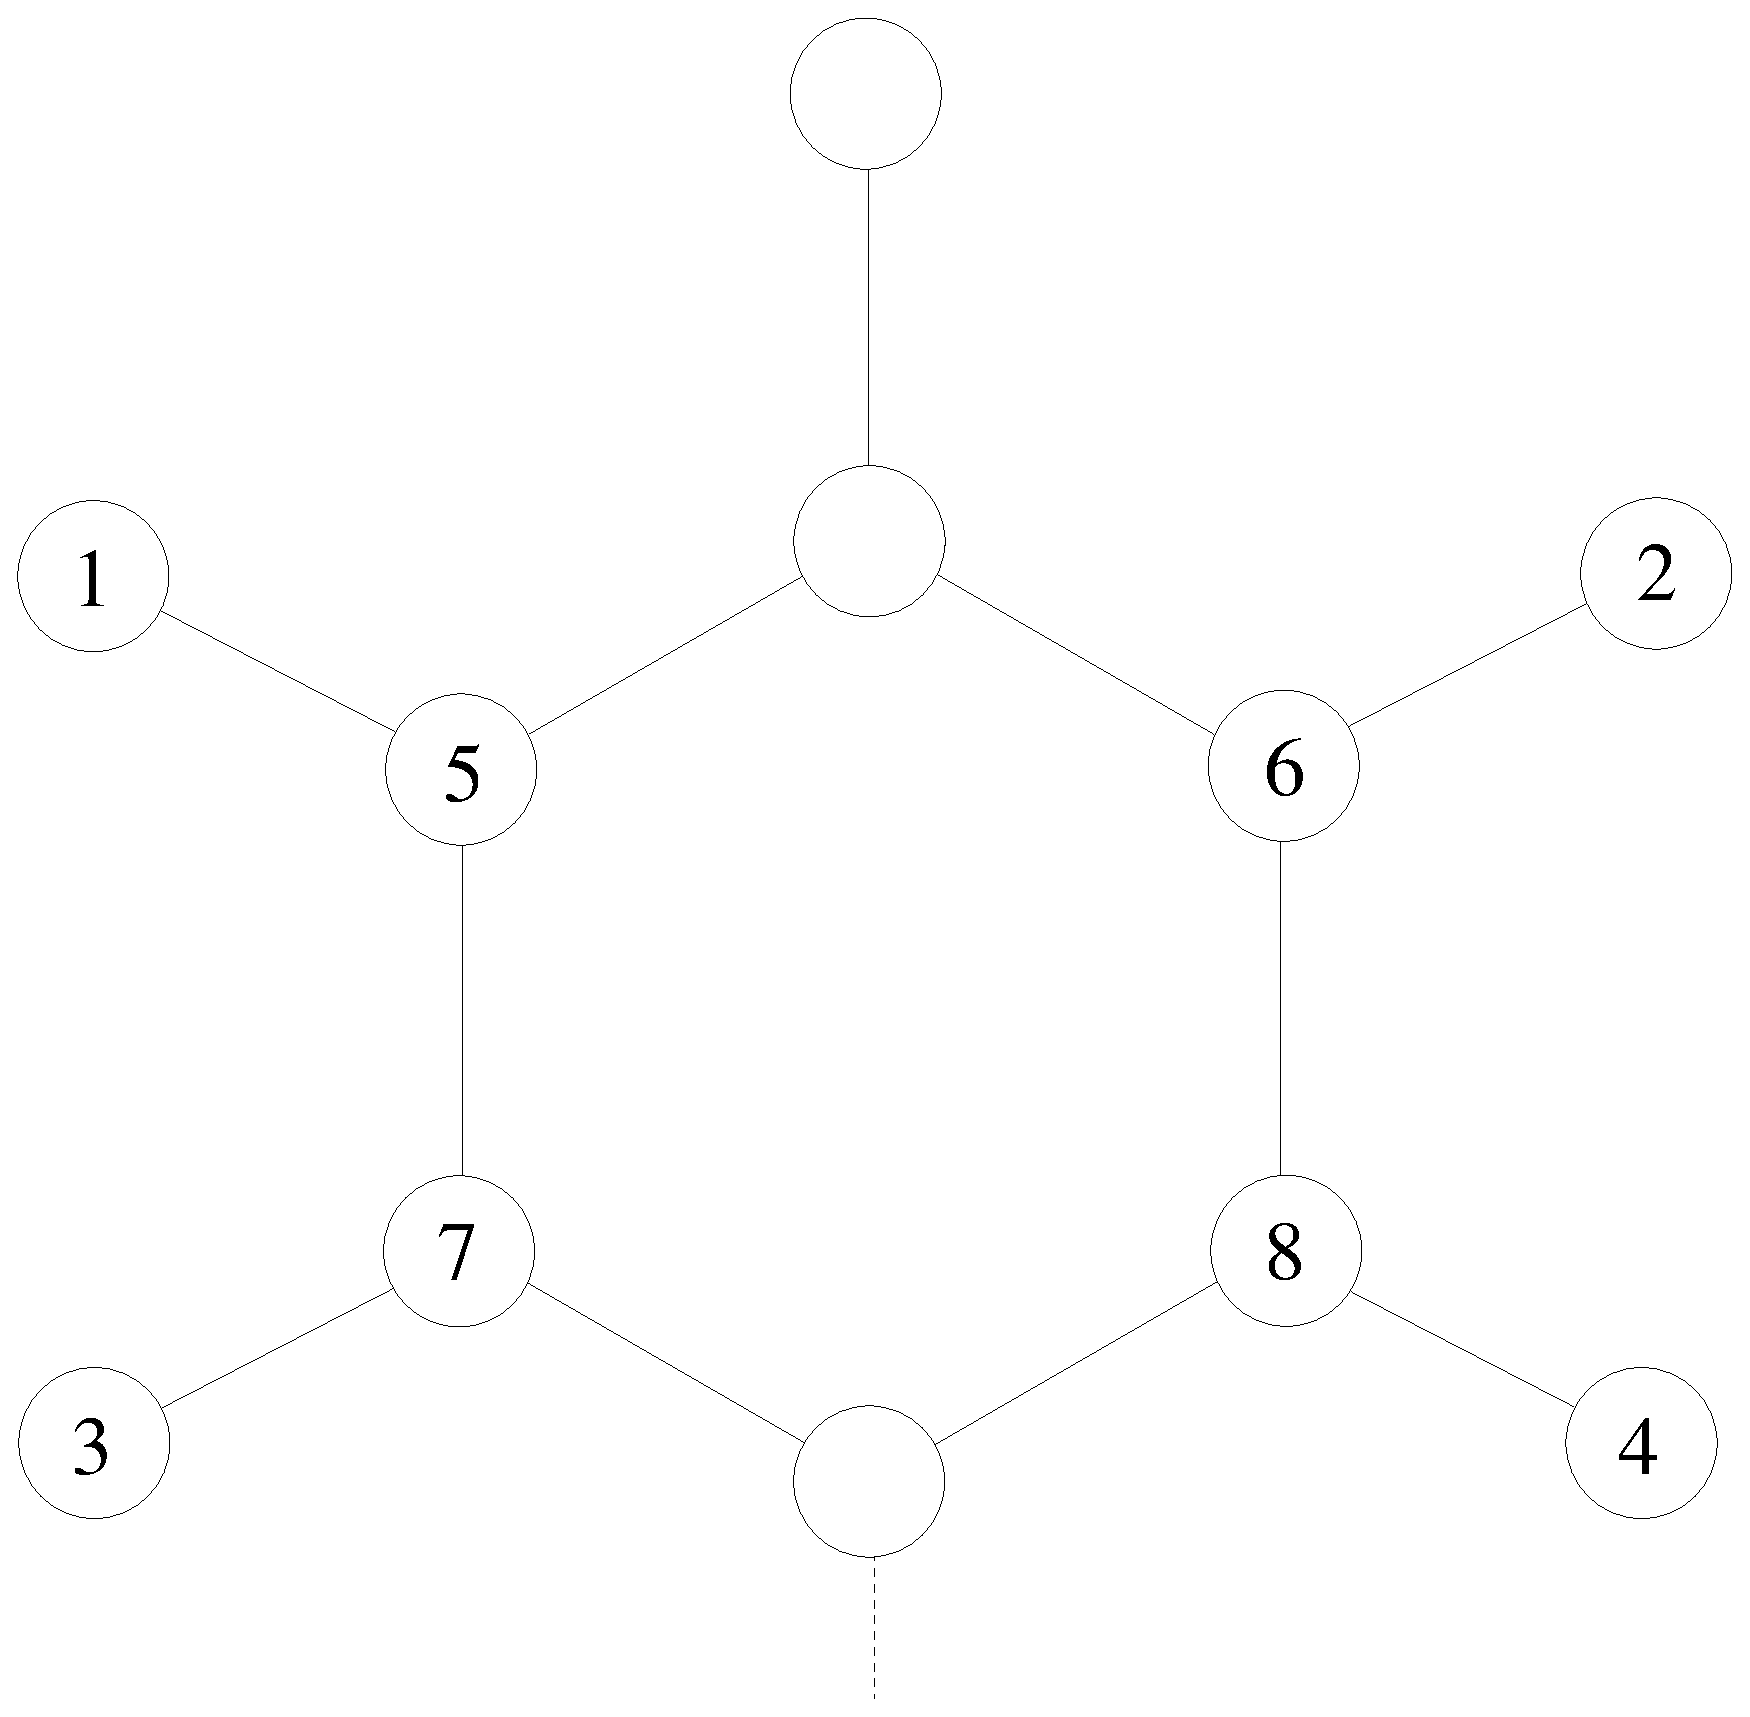
\includegraphics[width=0.5\textwidth]{PHE.eps}}
\end{figure}

For the phenylalanine example illustrated above we must allow three other pairs of
atoms to exchange if we swap 7 and 8. Hence a suitable {\tt perm.allow} entry is
{\obeylines
1
2 3
7 8 5 6 1 2 3 4
}
Here $n=2$ and $s=3$: if we exchange 7 and 8 then we must also exchange 5 and 6,
1 and 2, and 3 and 4. There are two atoms in each of the three secondary sets, 
since we have specified 7 and 8 as the two primary atoms.

Here is an example {\tt perm.allow} file for a water trimer using
the flexible {\keyw{QTIP4PF}\/} potential, where the energy is invariant to permutations
of water molecules and to exchanges of hydrogens in the same molecule. However,
hydrogens cannot exchange between different oxygens:
{\obeylines
4
3 2
1 4 7 2 3 5 6 8 9
2 0 
2 3
2 0 
5 6
2 0 
8 9
}
The first group of three oxygens has two atoms that must move with each oxygen,
i.e.~atoms 2 and 3 for oxygen 1, etc. Hydrogen permutations for each oxygen are
allowed by the three following groups. This scheme allows atoms to appear in more 
than one group. There must be a group containing each complete set of permutations
in order for permutation-inversion isomers to be recognised. The format
is compatible with an older scheme, where only pair swaps were allowed for
associated atoms, but now allows for more general permutations.

Scripts to generate allowed permutations automatically for CHARMM and AMBER are available from
the group web site. It is essential to use symmetrised versions of the corresponding
force fields! 

\ksec{PERMISOMER}{\/}: equivalent to {\keyw{PERMDIST}\/} above, expect that
distance minimisation 
with respect to permutational isomerisation is only carried out for stationary
points with energies that differ by less than the parameter specified by {\keyw{EDIFF}TOL}.
Hence permutational isomers should be identified, but the distance between minima with
different energies is not minimised with respect to atom permutations.
This option is provided for cases where the number of permutations is too 
minimise distances with respect to permutations in general.
Should be used with the {\keyw{PERMDIST}\/} keyword in {\tt OPTIM}.
The auxiliary file {\tt perm.allow} specifies which atoms may be permuted; see
{\keyw{PERMDIST}\/} above.
Note that the {\keyw{NATOMS}\/} keyword must precede {\it PERMISOMER\/} in the
{\tt pathdata} file.

\ksec{PERTURB}{ x\/}: initial maximum perturbation of the Cartesian coordinates of a minimum, 
when looking for a new connected minimum via a single-ended transition state search.

\ksec{PFOLD}{ n1 n2 x\/}: provides control parameters for the on-the-fly calculation
of committor probabilities during the construction of a stationary point database.
All new local minima are assigned an initial value of zero.
{\it n1} iterations are performed every {\it n2} cycles with parameter $\omega$ in
the successive overrelaxation equal to {\it x}.
Note that a valid solution also exists for all committor probabilities equal to unity.
I have seen the iteration converge to this solution for a  very small database that
has just been created with {\it DIJINIT\/}. 

\ksec{PLANCK}{ h\/}: specifies the value of Planck's constant in units of the
prevailing energy unit times seconds. This numerical value is required for 
regrouping free energies. For example, for the {\keyw{CHARMM}} potential $h$ needs
to be $9.546\times10^{-14}\,$s\,kcal/mol
See \S \ref{sec:units} for more details.


\ksec{PULL}{ \/}: add this keywork if the system has a non-zero static force 
added to the potential. {\tt PATHSAMPLE.2.1} only uses this keyword to determine the
number of zero Hessian eigenvalues (four). The attached atoms and force magnitude
are not required.

\ksec{PSCALE}{ x\/}: determines how the difference in committor probabilities,
$p$, is used to select the pair of minima used in the next attempted connection. If
$p/x > $ a random number drawn from $[0,1]$ then the distance criterion is accepted.
There is also a criterion for the minimum distance (see {\keyw{DSCALE}}).
If $p>x$ then the committor probability criterion is always satisfied; below $x$ the probability
of acceptance decreases linearly.

\subsection{R-Z}
\ksec{READMIN}{ file\/}: reads in the data for one or more minima from {\it file}
in {\tt OPTIM} min.data.info format and then stops. 
Any number of min.data.info files can be concatenated into {\it file}.
New entries will be created in {\tt min.data} and {\tt points.min}.
If {\tt min.A} and {\tt min.B} do not exist they are not created.
{\keyw{READMIN}} therefore provides an alternative way to start an initial
path calculation by providing minima, so long as {\tt min.A} and {\tt min.B}
are created by hand.
It also provides a way to add additional minima to an existing database, since
new entries should be appended. There is a check to make sure that the minima
added are different from all those currently known.

\ksec{REGROUP}{ x\/}: regroup the A and B sets using a disconnectivity graph 
analysis \cite{beckerk97,walesmw98,Wales03} at energy {\it x}. 
Any intervening minima that share a superbasin with an A or B minimum are reclassified
to belong to the A and B sets, respectively.\cite{TrygubenkoW06}
The number of minima and transition states {\it does not change}: only the
classification of minima as A or B is affected,
which will change any rate analysis that follows.
The corresponding
minima are printed in files {\tt min.A.regrouped} and {\tt min.B.regrouped}.

\ksec{REGROUPFREE}{ x\/}: the database will be regrouped by combining free
energy minima where forward and backward free energy barriers are both
less than {\it x}. Regrouping is performed iteratively until no further free
energy minima merge. 
In this scheme, groups that contain product and reactant minima
(A and B sets) are not allowed to merge. 
The regrouping continues even if product and reactant groups
could merge according to the barrier threshold: such mergers are simply forbidden.
Don't forget to assign an appropriate value for the Planck constant using the
{\keyw{PLANCK}\/} keyword. 
If one of the {\keyw{DIJKSTRA}}, {\keyw{SD}GT}, {\it SGT}, or {\it DGT} keywords is
present the corresponding analysis will be performed using the new groups
and free energies.

\ksec{REGROUPFREEAB}{ x\/}: the database will be regrouped as for
{\keyw{REGROUP}FREE\/} above, but only the A and B groups are changed.

\ksec{REGROUPPE}{ x\/}: the database will be regrouped based upon 
a superbasin analysis at potential energy $x$.
Minima will be reassigned as A and B-type if they are in a superbasin
with an A or B minimum for this threshold.
New files {\tt min.data.regrouped}, {\tt ts.data.regrouped}, {\tt min.A.regrouped}
and {\tt min.B.regrouped} will be created.
Don't forget to assign an appropriate value for the Planck constant using the
{\keyw{PLANCK}\/} keyword. See also {\keyw{REGROUP}RATE\/}.
{\keyw{REGROUP}PE\/} and {\keyw{REGROUP}RATE\/} are different from {\keyw{REGROUP}\/}
in that they actually change the internal database structure into free energy
minima and groups of transition states linking them.
In this scheme, groups that contain product and reactant minima
(A and B sets) are not allowed to merge. 
The regrouping continues even if product and reactant groups
could merge according to the barrier threshold: such mergers are simply forbidden.
If one of the {\keyw{DIJKSTRA}}, {\keyw{SD}GT}, {\it SGT}, or {\it DGT} keywords is
present the corresponding analysis will be performed using the new groups
and free energies.

\ksec{REGROUPRATE}{ x\/}: the database will be regrouped based upon harmonic transition
state theory rate constants. Minima are in the same group if they can interconvert
via a path that involves only rate constants greater than $x$.
Minima will be reassigned as A and B-type if they are in a group
with an A or B minimum for this threshold.
New files {\tt min.data.regrouped}, {\tt ts.data.regrouped}, {\tt min.A.regrouped}
and {\tt min.B.regrouped} will be created.
Don't forget to assign an appropriate value for the Planck constant using the
{\keyw{PLANCK}\/} keyword. See also {\keyw{REGROUP}PE\/}.
{\keyw{REGROUP}PE\/} and {\keyw{REGROUP}RATE\/} are different from {\keyw{REGROUP}\/}
in that they actually change the internal database structure into free energy
minima and groups of transition states linking them.
In this scheme, groups that contain product and reactant minima
(A and B sets) are not allowed to merge. 
The regrouping continues even if product and reactant groups
could merge according to the barrier threshold: such mergers are simply forbidden.
If one of the {\keyw{DIJKSTRA}}, {\keyw{SD}GT}, {\it SGT}, or {\it DGT} keywords is
present the corresponding analysis will be performed using the new groups
and free energies.

\ksec{REMOVESP}{\/}: the minima specified in files {\tt min.remove} and
{\tt ts.remove} are removed and new files {\tt min.data.removed},
{\tt ts.data.removed}, {\tt min.A.removed}, {\tt min.B.removed},
{\tt points.min.removed} and {\tt points.ts.removed}
are created with a consistent numbering scheme for the remaining stationary
points. The first lines of {\tt min.remove} and
{\tt ts.remove} must contain a single integer, which is the number of 
stationary points listed for removal on the remaining lines.

\ksec{RETAINSP}{\/}: minima {\bf not} specified in file {\tt min.retain} 
are removed and new files {\tt min.data.retained},
{\tt ts.data.retained}, {\tt min.A.retained}, {\tt min.B.retained},
{\tt points.min.retained} and {\tt points.ts.retained}
are created with a consistent numbering scheme for the remaining stationary
points. The first line of {\tt min.retain} 
must contain a single integer, which is the number of 
minima listed on the remaining lines.
Transition states are only retained if they link two minima specified in the
{\tt min.retain} file.

\ksec{REWEIGHT}{ nrwbins nrwreactant energyfile\/}: 
conditional probabilities of reactant minima are obtained from the quench
probabilities calculated using the energies in file {\tt energyfile}.
These energies could come from systematic quenching from an MD trajectory at
the same temperature, for example.
{\it nrwbins\/} is the number of bins to use in representing the quench
probability distribution and {\it nrwreactant} is the number of bins
to use in representing the minima in the reactant set.
This is a somewhat experimental option. Consult DJW before using!

\ksec{RIGIDBODIES}{ n\/}: specifies the number of rigid bodies; only one
of {\keyw{NATOMS}\/} and {\keyw{RIGIDBODIES}} should be present.

\ksec{SDGT}{ DisconnectSources AltPbb Rescale Normalise\/}: 
graph transformation rate calculation, which switches from sparse optimised to
dense optimised algorithms when the average number of connections
exceeds a certain threshold \cite{TrygubenkoW06}.
The four arguments are all logicals, so an example input line might look
\vbox{SDGT T T F F}. If true (the default) {\it DisconnectSources} specifies that
a full transformation should be performed for each source, disconnecting the 
other sources. The resulting rate constants correspond to the KMC result and
$k^{\rm KMC}$ \cite{Wales06}.
If {\it AltPbb\/} is true (default is false) then additional work is done to
maintain precision, which roughly doubles the execution time, but may be needed at low
temperature.
If {\it Rescale} is true (default false) an alternative strategy is used 
to try and prevent error propagation.
Setting {\it Normalise} true (default false) instructs {\tt GT2input.f90} to check the normalisation
of branch probabilities. This should not be necessary.

\ksec{SEED}{ n\/}: random number seed.

\ksec{SGT}{ DisconnectSources AltPbb Rescale Normalise\/}: 
sparse optimised graph transformation rate calculation \cite{TrygubenkoW06}.
The four arguments are all logicals, so an example input line might look
\vbox{SGT T T F F}. If true (the default) {\it DisconnectSources} specifies that
a full transformation should be performed for each source, disconnecting the 
other sources. The resulting rate constants correspond to the KMC result and
$k^{\rm KMC}$ \cite{Wales06}.
If {\it AltPbb\/} is true (default is false) then additional work is done to
maintain precision, which roughly doubles the execution time, but may be needed at low
temperature.
If {\it Rescale} is true (default false) an alternative strategy is used 
to try and prevent error propagation.
Setting {\it Normalise} true (default false) instructs {\tt GT2input.f90} to check the normalisation
of branch probabilities. This should not be necessary.

\ksec{SHORTCUT}{ minsep string\/}: try connecting minima that are further apart than {\it minsep\/}
steps on the best path, as calculated using Dijkstra's algorithm.
In the Dijkstra analysis minima with zero connections are removed. 
This value can be changed using a {\keyw{DIJKSTRA} n} line in {\tt pathdata}.
If the option argument {\it string\/} is set to {\it BARRIER\/} or {\it RATE\/} then
the strategy is different. We now look for pairs of minima on either side of
the highest barriers or minima linked by the smallest
rate constant on the best path, sorted according to the barrier height or the rate.
{\it minsep\/} is then used to define the largest number of steps away from 
the transition states for connection attempts.

\ksec{STARTFROMPATH}{ afile n1 n2 \/}: reads an initial path from file {\tt afile}. If this 
file is in {\keyw{DUMP}ALLPATHS} format then the keyword {\keyw{STAR}TTRIPLES} is also needed.
The files {\tt min.A} and {\tt min.B} are created: {\tt min.A} contains the entries
1 and {\it n1} and {\tt min.B} contains the entries 1 and {\it n2}.
If {\tt min.A} already exists then the run will terminate with a warning message
without overwriting it.

\ksec{STARTTRIPLES}{\/}: reads the initial path specified by
{\keyw{STAR}TFROMPATH a\/} from  file {\tt path.info.a} in the new {\keyw{DUMP}ALLPATHS}
format.

\ksec{SYSTEM}{ a\/}: the atom type label to be written to {\tt odata} files for {\tt OPTIM},
thus specifying the potential that {\tt OPTIM} will use.

\ksec{TAG}{ n x\/}: atom number {\it n\/} in the system is `tagged' by giving it 
an artificial mass {\it x\/}.

\ksec{TEMPERATURE}{ x\/}: specifies that the canonical ensemble at reduced temperature {\it x\/}
is to be used to calculate rate constants. Mutually exclusive with {\keyw{ENERGY}\/}.

\ksec{TRIPLES}{\/}: specifies that {\tt path.info} files read after startup 
have the new {\keyw{DUMP}ALLPATHS} format. Use {\keyw{STAR}TTRIPLES} and {\keyw{ADDTRIPLES}} to
read or add a single {\tt path.info} file in this format at the beginning of a run.

\ksec{TSTHRESH}{ x\/}: specifies that transition states above energy $x$ should
not be included in the database. Probably most useful with CHARMM, where genuine 
transition states with silly energies can certainly occur and give rise to underflow.

\ksec{TWOD}{\/}: the system is two-dimensional.

\ksec{UNRES}{\/}: specifies the UNRES potential.\cite{liwoopwrs97} % ,liwopwros97,liwokcgowrps98}

\ksec{UNTRAP}{ einc thresh\/}: try connecting minima to eliminate traps.
Connections are attempted between all minima and any of the minima in the
product set based on the largest barriers in the product direction, as estimated
from disconnectivity analysis at energy intervals of $einc$, starting from the
global minimum.
The product basin is defined as the set at the highest energy for which the 
minimum in question is not a member.
Candidate pairs of minima are sorted based upon the ratio of the
potential energy barrier to the potential energy difference between the minimum
in question and the lowest product minimum.
Hence this scheme is analogous to the {\keyw{FREEPAIRS}\/} procedure, but
uses individual minima and potential energy, instead of free energy.
Minima from the product basin above energy $thresh$ will only be considered if there
are no minima below this threshold.
In a second phase the original product minimum may be replaced by a minimum from
the same superbasin that is closer to the target minimum, so long as its energy
lies below the threshold.
Minima with zero connections are not considered; 
this value can be changed using a {\keyw{DIJKSTRA} n} line in {\tt pathdata}, even
though a Dijkstra analysis is not used.
See also the {\keyw{PAIRLIST}\/} keyword.
The {\keyw{UNTRAP} \/} keyword may provide the best way to remove artificial 
frustration from potential energy disconnectivity graphs.
It may be helpful to choose a larger value of {\it einc\/} than would be
used for the superbasin analysis in visualising the disconnectivity graph.
This will encourage connection attempts with minima of lower energy in the
expanded product superbasin. 

\ksec{USEPAIRS}{ Epathfile\/}: pairs of minima are chosen for connection attempts based
on the order of local minima specified in file {\tt Epathfile}, which must have the format
of a {\tt PATHSAMPLE} {\tt Epath} output file 9as generated by {\keyw{DIJKSTRA}\/}, etc.
This keyword is intended to follow a {\keyw{DUMMYTS}\/} run, where the stationary point
database has been refined using {\keyw{BHINTERP}\/} or {\keyw{BISECT}\/} runs in {\tt OPTIM}.
The dummy {\tt ts.data} and {\tt pairs.data} files must be renamed or removed
before the {\keyw{USEPAIRS}\/} run.
The pairs of minima are first chosen to be the adjacent structures from the list, then
second-neighbours, until all possible pairs have been tried.


\section{{\tt odata} files}
\label{sec:odatafiles}

The following {\tt odata} template
files may be necessary, one for each type of {\tt OPTIM} job which can be launched by {\tt PATHSAMPLE}.
If {\keyw{CONNECT}IONS} is set to one or fewer then only an {\tt odata.connect} template is
needed.
\smallskip
\begin{itemize}
\item {\tt odata.connect}: the template file for double-ended pathway searches.

\item {\tt odata.path}: template for pathway calculations to find the two minima connected by
steepest-descent paths to a single transition state. Reads in the eigenvector corresponding to
the negative eigenvalue (transition mode) from file {\tt vector.dump} produced by {\tt odata.tssearch}.

\item {\tt odata.tssearch}: performs a single-ended transition state search.

\end{itemize}

Please refer to the {\tt OPTIM} manual\cite{optim} for details of {\tt odata} files.
In the templates the {\tt odata} file should not contain any coordinates, and should terminate
with the {\it POINTS} or {\keyw{CHARMM}} keyword, as appropriate.
\pagebreak

\section{Output files}
\label{sec:output}

{\tt PATHSAMPLE} produces information about its progress on standard output;
more details can be obtained with the {\keyw{DEBUG}} keyword. 
The databases of minima and
transition states ({\tt min.data}, {\tt ts.data}, {\tt points.min} and {\tt points.ts}) described in
\S\ref{sec:input} are updated as necessary. 

\section{ A Note on Units and Planck's Constant}
\label{sec:units}

Aside from {\keyw{CHARMM}} and {\keyw{AMBER}} {\tt OPTIM} does no
unit conversions. These systems are treated differently, as explained below.
For all other cases {\tt PATHSAMPLE} is
expecting to receive $\ln\Pi_i \omega^2_i$ in the {\tt min.data}
and {\tt ts.data} files. {\tt PATHSAMPLE} converts $\omega$ to
$\nu$ using $\nu=\omega/2\pi$, but also does no unit conversions.
The rate constants are therefore in natural frequency units of
$\sqrt{\epsilon/m\sigma^2}$, where $\epsilon$ is the unit of energy,
$m$ is the unit of mass, and $\sigma$ is the unit of length.

For a system where all particles have equal masses, $m$, the rate constants
calculated by {\tt PATHSAMPLE} can therefore be converted to SI units
by multiplying by $\sqrt{(\epsilon/{\rm J})/(m/{\rm kg})(\sigma/{\rm m})^2}$.

For calculations involving free energy regrouping schemes we need to supply
a value for the Planck constant in reduced units via the {\keyw{PLANCK}} keyword.
Since the temperature is read in energy units, i.e.~$\epsilon$, so that $k_BT$
is in $\epsilon$, we need to define $h$ in reduced units so that terms like
$k_BT/h\nu$ are dimensionless. If $\nu$ is in reduced time units then we
need $(h/{\rm Js})$ divided by the unit of energy and the unit of time. 
The reduced value of $h$ is therefore
\begin{equation}
\frac{(h/{\rm Js})}{(\epsilon/{\rm J})
\sqrt{\displaystyle\frac{(m/{\rm kg})(\sigma/{\rm m})^2}{(\epsilon/{\rm J})}}} 
= \frac{(h/{\rm Js})}{\sqrt{(m/{\rm kg})(\sigma/{\rm m})^2(\epsilon/{\rm J})}}.
\end{equation}

For {\keyw{CHARMM}} and {\keyw{AMBER}} we need to diagonalise the reciprocal
mass-weighted Hessian in {\tt OPTIM}, where the various masses are known.
For convenience the frequency unit conversion is done in {\tt OPTIM} as
well, so that the rate constants calculated in {\tt PATHSAMPLE} are
in s$^{-1}$ and do not need to be converted.
The value required for the Planck constant is therefore different because
$\nu$ is not in reduced units. Instead, we need to convert $(h/{\rm Js})(\nu/{\rm s}^{-1})$
to kcal/mol, since these are the units of $k_BT$. Hence we need $(h/{\rm Js})/(\epsilon/{\rm J})$,
where $\epsilon$ is one kcal/mol. Since 1\,kcal/mol is $6.948\times10^{-21}\,$J
the required value for the {\keyw{PLANCK}\/} keyword in regrouping calculations
is $6.626\times10^{-34}/6.948\times10^{-21}=9.536\times10^{-14}$.


\section{Known Problems}
\label{sec:problems}

If all {\tt OPTIM} jobs are failing for some reason then it is likely
that the rsh command that starts the jobs on remote nodes will run out of
sockets. Using a single rsh command together with cp via nfs to copy results
back seems to have eliminated the previous problems that we sometimes saw
with socket errors.

Rate constant calculations with any graph transformation variant can be very
memory hungry. They will die with a segmentation fault if they run out
of memory.

%<examples>
\section{Example {\tt pathdata} files}
\label{sec:example}
\subsection{Starting from an {\tt OPTIM} {\tt path.info} file}

The following {\tt pathdata} file was used on a distributed memory machine.
It loads an initial path from {\tt path.info.startup} and creates {\tt min.A}
and {\tt min.B} files containing the entries 1 and 9 and 1 and 16, respectively.
1000 iterations of the committor probabilities are performed every cycle,
removing minima with one connection or fewer, and using a successive
overrelaxation parameter of 1.99.
Rate constants are calculated using graph transformation every 10 cycles,
again removing minima with one connection or fewer.
\medskip

\begin{table}[H]
\begin{center}
\begin{tabular}{ll}
JOBSPERNODE & 2 \\
NATOMS       &  56 \\
SYSTEM        & BL \\
STARTFROMPATH & startup 9 16 \\
COMMENT & ADDPATH add \\
GT & 1 10 \\
TEMPERATURE&    0.42 \\
DSCALE      &    3.0 \\
PSCALE       &   1.0 \\
PFOLD         &  1000 1 1.99 \\
CYCLES      &    500 \\
CONNECTIONS  &  1 \\
SEED      &     1 \\
PERTURB    &    0.3D0 \\
ETOL        &   0.0000005D0 \\
ITOL        &   0.1 \\
DIRECTION    &  AB \\
EXEC        &   /home/wales/bin/OPTIM.3.2 \\
TRIPLES & \\
STARTTRIPLES & 
\end{tabular}
\end{center}
\end{table}

\subsection{Starting from {\tt OPTIM} {\tt min.data.info} files}

It is also possible to start {\tt PATHSAMPLE} runs without an existing 
connection between the end points of interest. See keywords {\keyw{DIJINITSTART}\/}
and {\keyw{DIJINITCONT}\/}.
In this example we set up {\tt PATHSAMPLE} from {\tt min.data.info} files for the 
two minima and use {\keyw{DIJINITCONT}\/} to continue the run and seek an initial 
connection using {\tt PATHSAMPLE}.

First, a minimisation was run for each minimum using {\tt OPTIM} with the
{\keyw{DUMP}DATA} keyword set. The {\keyw{ENDHESS}} keyword was used to produce frequencies after a
{\keyw{BFGS}MIN\/} optimisation.
In a clean directory, with no preexisting {\tt PATHSAMPLE} files, two entries were created
in {\tt min.data} and {\tt points.min} using the {\tt PATHSAMPLE} {\keyw{READMIN}\/} keyword
to read each of the {\tt min.data.info} files in turn. {\tt min.A} and {\tt min.B} files were
then created using vi with one entry in each, pointing to minima 1 and 2, respectively. 
After creating a suitable {\tt odata.connect} file a single cycle of {\tt PATHSAMPLE}
was then run on one core to populate the database with enough minima to run on
multiple cores in subsequent connection attempts. Since there is only one possible connection
to try in the first cycle, it is necessary to use a single processor in this case
along with the {\keyw{DIJINITCONT}\/} keyword in {\tt pathdata}. A couple of cycles on
eight cores then produced a connection for this bulk BLJ$_{60}$ example.
\medskip

\begin{table}[H]
\begin{center}
\begin{tabular}{ll}
NATOMS   &      60 \\
COPYFILES & perm.allow \\
BULK  & 3.587037905 3.587037905 3.587037905 \\
PERMDIST \\
SYSTEM  &       LS \\
TEMPERATURE &   0.71 \\
CONNECTIONS &   1 \\
SEED        &   1 \\
PERTURB     &   0.40 \\
ETOL        &   1.0D-7  \\
ITOL        &   1.1D0 \\
GEOMDIFFTOL        &   0.1D0  \\
DIRECTION   &   AB \\
EXEC        &  /home/wales/bin/OPTIM \\
TRIPLES &  \\
ADDTRIPLES &  \\
STARTTRIPLES &  \\
 & \\
comment READMIN min.data.info.start \\
comment READMIN min.data.info.finish \\
comment CPUS 1 \\
 & \\
DIJINITCONT EXP \\
CYCLES        100 \\
JOBSPERNODE 1 \\
PAIRLIST 1
\end{tabular}
\end{center}
\end{table}
\medskip

The commented lines were used to read in the initial {\tt min.data.info} files.
A similar procedure can be used if an initial {\tt path.info} file is available
without a complete connection between the desired end points.


